\documentclass[conference]{IEEEtran}
\IEEEoverridecommandlockouts
\usepackage{cite}
\usepackage{amsmath,amssymb,amsfonts,bm}
\usepackage{graphicx}
\usepackage{booktabs}
\usepackage{xcolor}
\usepackage{url}
\renewcommand{\boldsymbol}{\bm}
% Framed placeholder for figures to be inserted later
\newcommand{\figplaceholder}[2]{\fbox{\parbox[c][#1][c]{0.97#2}{\centering\color{gray}\footnotesize Reserved space for figure}}}
\begin{document}
\title{Nalanda AI: Grounded Sequence-to-Sequence Answer Refinement and Autoencoder-Based Scope Detection for Edge-Hosted Academic Study}
\author{\IEEEauthorblockN{Sayali Rajput}
\IEEEauthorblockA{\textit{B.Tech. in Artificial Intelligence and Data Science (AI-DS)}\\SVKM's Narsee Monjee Institute of Management Studies (NMIMS)\\Navi Mumbai, Maharashtra, India\\rajput174@nmims.in}
\and
\IEEEauthorblockN{Mayank Sawant}
\IEEEauthorblockA{\textit{B.Tech. in Artificial Intelligence and Data Science (AI-DS)}\\SVKM's Narsee Monjee Institute of Management Studies (NMIMS)\\Navi Mumbai, Maharashtra, India\\mayank.sawant049@nmims.in}}
\maketitle
\begin{abstract}Students increasingly revise from lecture slides with retrieval-augmented assistants, yet such systems can return fragmented passages, introduce content that is absent from the source, answer questions outside the course scope, and generate implausible self-test items. This paper presents Nalanda AI, a locally hosted study workspace that combines dense retrieval over all-MiniLM-L6-v2 embeddings, FLAN-T5-small answer refinement protected by a lexical and entity-level grounding check with extractive fallback, a per-folder undercomplete autoencoder that flags out-of-scope queries through reconstruction error, and a quiz generator that selects distractors inside a cosine-similarity band. The components are evaluated on 253 chunks from three Big Data Analytics lecture decks, with a separate course (62 chunks) and 50 probe queries serving as out-of-distribution data. Across five random splits, principal component analysis with $k=32$ achieved lower held-out reconstruction error than the deployed 35-epoch autoencoder (0.75 vs. 2.37 $\times 10^{-3}$). The autoencoder detector separated off-topic from in-domain queries with an AUROC of 0.990, although a PCA-residual detector performed at least as well (0.999). On a five-question answer-refinement benchmark, the pipeline produced no unsupported entities under the project's entity metric and correctly abstained on the unanswerable question; however, on the four answerable questions its token F1 (0.413) was below that of direct extraction (0.532). All 104 automated software tests pass. The results support the scope-detection and abstention components, while indicating that generative refinement requires larger-scale evaluation before improvements in answer quality can be claimed.\end{abstract}
\begin{IEEEkeywords}Retrieval-augmented generation, sequence-to-sequence models, autoencoders, principal component analysis, out-of-distribution detection, question generation, educational technology\end{IEEEkeywords}
\section{Introduction}
Active retrieval practice improves long-term retention more than re-reading \cite{roediger2006}, and learners frequently overestimate how well they understand complex mechanisms until they are asked to explain them \cite{rozenblit2002}. Study tools that let a student question their own lecture material, and then test themselves on it, are therefore pedagogically attractive. Retrieval-augmented generation (RAG) provides a natural technical basis for such tools: relevant passages are retrieved from a document collection and passed to a generative model that composes an answer \cite{lewis2020,gao2023}.

Applying RAG to university lecture slides exposes several practical problems. First, slide decks are terse and fragmented, so the top-ranked chunk often contains only part of an enumeration or procedure. Second, generative models can produce statements that are not supported by the retrieved evidence \cite{maynez2020,ji2023}, which is particularly harmful when the student intends to reproduce the answer in an examination. Third, a general-purpose model will usually answer questions unrelated to the course instead of reporting that the material does not cover them. Fourth, automatically generated multiple-choice questions depend heavily on distractor quality: options that are synonyms of the key make an item ambiguous, whereas options from an unrelated domain make it trivial \cite{mitkov2003,kurdi2020}. Finally, many institutions prefer that course material and student interaction logs remain on local infrastructure rather than being sent to commercial cloud services.

This paper describes \emph{Nalanda AI}, a study workspace that addresses these problems with small models that run on a laptop-class machine and with transparent, rule-based safeguards around them. The system does not introduce a new learning algorithm; its contribution lies in the integration of established techniques and in an evaluation that compares each learned component with a simpler baseline. Specifically, this paper makes the following contributions:

\begin{enumerate}
\item A description of an end-to-end, document-scoped study system combining dense retrieval, FLAN-T5 answer refinement with a grounding check and extractive fallback, autoencoder-based scope detection, and cosine-constrained distractor selection, with each component traced to its implementation.
\item A reproducible comparison of principal component analysis (PCA) and the deployed undercomplete autoencoder on real lecture embeddings, using held-out data, five random splits, and five latent sizes.
\item An evaluation of reconstruction-error out-of-distribution (OOD) detection against PCA-residual and centroid-distance baselines on cross-course chunks and probe queries.
\item A per-case analysis of the project's answer-refinement benchmark that identifies where its aggregate gains originate, together with an audit of discrepancies between the project documentation and the code.
\end{enumerate}
Section~II reviews related work and Section~III formulates the problem. Section~IV describes the architecture and Section~V the experimental methodology. Section~VI defines the metrics, Section~VII reports results, and Sections~VIII--X discuss the findings, limitations, and future work.

\section{Related Work}
\subsection{Retrieval-Augmented Generation and Sentence Embeddings}
Lewis \emph{et al.} \cite{lewis2020} combined a dense retriever with a sequence-to-sequence generator and showed gains on knowledge-intensive tasks; dense passage retrieval \cite{karpukhin2020} established bi-encoder retrieval as a strong alternative to sparse methods, and Gao \emph{et al.} \cite{gao2023} survey the subsequent design space. Sentence-BERT \cite{reimers2019} made bi-encoder sentence embeddings efficient enough for semantic search, and MiniLM \cite{wang2020} distilled such encoders into compact models. Nalanda AI uses the all-MiniLM-L6-v2 checkpoint, which follows this line of work, to embed both chunks and queries.

\subsection{Encoder--Decoder Transformers}
The Transformer \cite{vaswani2017} replaced recurrence with multi-head attention. T5 \cite{raffel2020} cast NLP tasks in a text-to-text format and replaced absolute position embeddings with learned, bucketed relative position biases, a refinement of relative position representations \cite{shaw2018}. FLAN-T5 \cite{chung2024} further instruction-tuned T5 on a large task mixture, improving zero-shot instruction following. The present system uses the smallest FLAN-T5 checkpoint so that inference remains feasible without a discrete GPU.

\subsection{Dimensionality Reduction and Autoencoders}
PCA \cite{pearson1901,jolliffe2016} projects data onto the directions of maximal variance; by the Eckart--Young theorem \cite{eckart1936}, the truncated singular value decomposition gives the best rank-$k$ approximation in the least-squares sense. Baldi and Hornik \cite{baldi1989} showed that a linear autoencoder trained with squared error recovers the principal subspace, so nonlinear autoencoders \cite{hinton2006} can only improve on PCA by exploiting curvature in the data manifold. Variational autoencoders \cite{kingma2014} impose a probabilistic latent prior, and denoising autoencoders \cite{vincent2008} learn to map corrupted inputs back to clean ones.

\subsection{Anomaly and Out-of-Distribution Detection}
Chandola \emph{et al.} \cite{chandola2009} review anomaly detection, including reconstruction-based approaches. Sakurada and Yairi \cite{sakurada2014} used autoencoder reconstruction error to detect anomalies and compared it with linear PCA, and Hendrycks and Gimpel \cite{hendrycks2017} established simple baselines and AUROC-based evaluation for OOD detection. These works motivate the comparison of autoencoder and PCA residuals in Section~VII.

\subsection{Question Generation and Distractor Selection}
Mitkov and Ha \cite{mitkov2003} generated multiple-choice items by selecting semantically close concepts as distractors, and Kurdi \emph{et al.} \cite{kurdi2020} systematically reviewed automatic question generation for education, noting that evaluation is often limited and rarely includes psychometric analysis. Nalanda AI follows the similarity-based approach to distractor selection.

\subsection{Faithfulness of Generated Text}
Maynez \emph{et al.} \cite{maynez2020} showed that abstractive models frequently produce unfaithful content, and Ji \emph{et al.} \cite{ji2023} survey hallucination across generation tasks. Lexical overlap metrics such as token F1 \cite{rajpurkar2016} and ROUGE-L \cite{lin2004} are inexpensive but correlate imperfectly with faithfulness. The grounding check in this work is a lightweight lexical heuristic and should be interpreted in that light.

\section{Problem Formulation and Research Objectives}
Let a course folder contain chunks $\mathcal{D}=\{c_1,\dots,c_N\}$ extracted from uploaded documents, each with a unit-norm embedding $\mathbf{e}_i\in\mathbb{R}^{384}$. Given a student query $q$, the system must (i) return an answer $a$ whose content is supported by retrieved evidence $\mathcal{E}\subset\mathcal{D}$, or abstain; (ii) identify queries and documents that lie outside the scope of the folder; and (iii) produce multiple-choice items whose distractors are plausible but not equivalent to the key. These tasks must run on a single local machine and remain isolated per user and per folder. The evaluation addresses four research questions:

\begin{itemize}
\item \textbf{RQ1:} How does linear PCA compare with the deployed undercomplete autoencoder in held-out reconstruction fidelity and computational cost on lecture embeddings?
\item \textbf{RQ2:} Does autoencoder reconstruction error separate in-scope from out-of-scope chunks and queries, and how does it compare with simpler detectors?
\item \textbf{RQ3:} Does grounded refinement reduce unsupported content relative to an unguarded sequence-to-sequence baseline, and how does it affect lexical agreement with reference answers?
\item \textbf{RQ4:} How does the implemented cosine band partition the space of candidate distractor concepts?
\end{itemize}
Models are executed locally once downloaded; the model weights themselves are obtained from the Hugging Face Hub on first use, so the system is not free of external dependencies at installation time.

\section{Proposed System Architecture}
Fig.~\ref{fig:arch} summarizes the architecture. A browser client communicates with a FastAPI server that manages users, folders, and documents in SQLite through SQLAlchemy. Each folder has an isolated vector index. Retrieval results flow to the answer-refinement, notes, and quiz services; the autoencoder detector operates on the same embeddings. The following subsections describe each component as implemented in the project source code.

\begin{figure*}[!t]
\centering
\figplaceholder{2.6in}{\textwidth}
\caption{Overall architecture of Nalanda AI: client views, API layer, per-folder vector index, and the refinement, scope-detection, notes, and quiz services.}
\label{fig:arch}
\end{figure*}
\subsection{Document Ingestion and Text Normalization}
Digital PDF pages are parsed with PyMuPDF, which extracts text, native tables, and raster figures; pages without an extractable text layer, and standalone images, are processed with PaddleOCR (PP-StructureV3). Extraction runs in a time-limited subprocess. Regular-expression normalization then repairs line-break hyphenation, unwraps soft line breaks, removes repeated slide banners, and protects code blocks and tables. Text is grouped into section-aware chunks of roughly 1{,}200--1{,}800 characters with a 150-character overlap, and each chunk retains its document identifier, page number, section title, and links to figures and tables (Fig.~\ref{fig:pipeline}).

\begin{figure}[!t]
\centering
\figplaceholder{2.3in}{\columnwidth}
\caption{Document ingestion and retrieval pipeline, from upload and extraction to normalization, chunking, embedding, and per-folder indexing.}
\label{fig:pipeline}
\end{figure}
\subsection{Semantic Embedding and Retrieval}
Chunks and queries are encoded with all-MiniLM-L6-v2 \cite{wang2020,reimers2019} and L2-normalized, so that the dot product equals cosine similarity. Embeddings are stored per folder as a NumPy matrix with a JSON metadata file, and retrieval ranks chunks by dot product with the query vector. Adjacent chunks belonging to the same section are stitched together before answer generation to reduce fragmentation.

\subsection{Dimensionality Reduction with PCA}
For a matrix of $N$ embeddings $\mathbf{X}\in\mathbb{R}^{N\times D}$ with mean $\bar{\mathbf{x}}$, PCA is computed from the singular value decomposition of the centered data:

\begin{equation}
\mathbf{X}_c=\mathbf{X}-\mathbf{1}\bar{\mathbf{x}}^{\top}=\mathbf{U}\mathbf{\Sigma}\mathbf{V}^{\top}
\label{eq:svd}
\end{equation}
Retaining the first $k$ right singular vectors $\mathbf{V}_k$ yields the reconstruction and the explained-variance ratio

\begin{equation}
\hat{\mathbf{X}}=\mathbf{X}_c\mathbf{V}_k\mathbf{V}_k^{\top}+\mathbf{1}\bar{\mathbf{x}}^{\top},\qquad \eta_k=\frac{\sum_{i=1}^{k}\sigma_i^2}{\sum_{j}\sigma_j^2}
\label{eq:pca}
\end{equation}
In the current implementation, PCA is provided as a benchmarking utility and is not part of the request-serving path; Section~VII evaluates it both as a compressor and as an OOD scoring function.

\subsection{Autoencoder-Based Scope Detection}
The deployed detector is an undercomplete autoencoder with encoder $384\rightarrow128\rightarrow k$ and a mirrored decoder, using layer normalization \cite{ba2016}, LeakyReLU (slope 0.2), dropout of 0.05, and a layer-normalized latent code with $k=32$. With encoder $f_\theta$ and decoder $g_\phi$,

\begin{equation}
\mathbf{z}=f_\theta(\mathbf{x}),\qquad \hat{\mathbf{x}}=g_\phi(\mathbf{z}),\qquad \mathcal{L}_{\mathrm{AE}}=\frac{1}{D}\|\mathbf{x}-\hat{\mathbf{x}}\|_2^2
\label{eq:ae}
\end{equation}
A separate model is trained for each folder on all of its chunk embeddings, using full-batch Adam \cite{kingma2015} with a learning rate of $5\times10^{-3}$, weight decay of $10^{-5}$, and 35 epochs, and is cached on disk. For a query embedding $\mathbf{q}$, the reconstruction error is

\begin{equation}
e(\mathbf{q})=\frac{1}{D}\|\mathbf{q}-g_\phi(f_\theta(\mathbf{q}))\|_2^2
\label{eq:err}
\end{equation}
Let $\bar{e}$ and $s_e$ be the mean and standard deviation of the training errors. The query is flagged when

\begin{equation}
e(\mathbf{q})>\bar{e}+3\max(s_e,\,5\times10^{-4})\ \ \vee\ \ (e(\mathbf{q})-\bar{e})/s_e\geq 3
\label{eq:rule}
\end{equation}
The search service returns an out-of-scope message only if the query is flagged \emph{and} the best retrieval similarity is below 0.28. During ingestion, a new document is marked as mismatched in its metadata, without being rejected, when at least 65\% of its chunks are flagged. The code base also contains a variational autoencoder \cite{kingma2014} trained on the negative evidence lower bound

\begin{equation}
\mathcal{L}_{\mathrm{VAE}}=\frac{1}{D}\|\mathbf{x}-g_\phi(\mathbf{z})\|_2^2-\frac{\beta}{2}\sum_{j=1}^{k}\left(1+\log\sigma_j^2-\mu_j^2-\sigma_j^2\right)
\label{eq:vae}
\end{equation}
with $\mathbf{z}=\boldsymbol{\mu}+\boldsymbol{\sigma}\odot\boldsymbol{\epsilon}$ and $\boldsymbol{\epsilon}\sim\mathcal{N}(\mathbf{0},\mathbf{I})$, a denoising autoencoder \cite{vincent2008} (Gaussian noise $\sigma=0.15$, feature masking $p=0.10$, latent size 48), and a sparse autoencoder with an L1 penalty. These variants are implemented and unit-tested, but in the evaluated version none of them is invoked in the serving or ingestion path.

\subsection{Sequence-to-Sequence Answer Refinement}
Answer refinement uses FLAN-T5-small \cite{chung2024,raffel2020}: an encoder--decoder Transformer with eight encoder and eight decoder layers, model width 512, six attention heads of dimension 64, gated-GELU feed-forward layers, and approximately 77M parameters. T5 attention omits explicit $1/\sqrt{d_k}$ scaling and adds a learned scalar bias that depends on the bucketed relative distance between positions (32 buckets):

\begin{equation}
\mathrm{Attn}(\mathbf{Q},\mathbf{K},\mathbf{V})=\mathrm{softmax}(\mathbf{Q}\mathbf{K}^{\top}+\mathbf{B})\mathbf{V},\qquad B_{ij}=b_h(\mathrm{bkt}(j-i))
\label{eq:attn}
\end{equation}
Up to six retrieved chunks form the context. Generation uses beam search with two beams, a no-repeat $n$-gram size of 3, and minimum and maximum output lengths of 32 and 1{,}536 tokens; the configured maximum input length is 2{,}048 tokens, which exceeds the 512-token length used in T5 pre-training. Before generation, a deterministic structurer classifies the query as procedural, taxonomic, comparative, or descriptive and formats the evidence as numbered steps, bullet lists, comparison tables, or paragraphs respectively; this structured evidence also serves as the extractive fallback.

\subsection{Entity-Level Grounding and Extractive Fallback}
Each candidate answer $a$ is sanitized (conversational preambles, slide numbering, and OCR artifacts are removed) and compared with the concatenated evidence. Let $T(\cdot)$ denote the set of non-stop-word content tokens and $\mathcal{M}(a)$ the set of entities in $a$, where entities are acronyms or multi-word title-case phrases detected by a regular expression. The check computes the token overlap and the unsupported-entity ratio

\begin{equation}
\rho=\frac{|T(a)\cap T(\mathcal{E})|}{|T(a)|},\qquad u=\frac{|\{m\in\mathcal{M}(a):m\notin\mathcal{E}\}|}{|\mathcal{M}(a)|}
\label{eq:ground}
\end{equation}
and a composite confidence that also uses the retrieval confidence $r$:

\begin{equation}
c=\left(0.6\,\rho+0.4\,(1-u)\right)\min(1,\,r+0.2)
\label{eq:conf}
\end{equation}
An answer is accepted when $\rho\geq0.35$, $c\geq0.40$, no repetition loop is detected, and it is not the case that $u>0.45$ with at least two unsupported entities. Otherwise, the structured extractive answer is validated in the same way and returned if its confidence is higher. If $r<0.30$ or fewer than 15\% of query tokens occur in the evidence, the system abstains with a fixed message. This procedure is a heuristic filter, not a formal guarantee: a single unsupported entity, a substituted lowercase word, or an unsupported claim phrased with supported vocabulary can pass.

\subsection{Geometry-Constrained Multiple-Choice Question Generation}
The quiz generator mines fact anchors from chunks using copular and enumerative patterns (for example, ``$X$ is defined as $Y$'') and converts each anchor into a question stem whose key is the anchor concept. Candidate distractors come from concepts in the folder and from curated lists of sibling concepts per domain. With $\mathbf{e}_a$ and $\mathbf{e}_d$ the MiniLM embeddings of the key and a candidate, the eligible set is

\begin{equation}
\mathcal{D}(a)=\{d\in\mathcal{C}:\ 0.25\leq\cos(\mathbf{e}_a,\mathbf{e}_d)<0.92\}
\label{eq:band}
\end{equation}
The upper bound excludes near-synonyms of the key and the lower bound excludes unrelated concepts. Eligible candidates are ranked by decreasing similarity, and string-level rules remove options that are too similar to the key or to each other. If fewer than three distractors remain, curated siblings are added; if the pool is still insufficient, FLAN-T5 is prompted to list related concepts. The procedure is therefore primarily geometric but not entirely non-generative.

\subsection{Full-Stack Application Integration}
The client is a single-page application written in HTML, CSS, and JavaScript with four views (Fig.~\ref{fig:ui}): a home dashboard; a conversational question-answering view with source citations and page previews; a notes view that assembles multi-document study notes and exports them to PDF; and a quiz view that presents ten-question multiple-choice quizzes with feedback and page references.

\begin{figure*}[!t]
\centering
\figplaceholder{2.8in}{\textwidth}
\caption{Nalanda AI user interface: home dashboard, conversational question answering with citations, study-notes view with PDF export, and practice-quiz view.}
\label{fig:ui}
\end{figure*}
\section{Experimental Methodology}
\subsection{Data}
The in-distribution corpus consists of the 253 stored chunk embeddings of one course folder containing three Big Data Analytics lecture decks (65, 116, and 72 chunks, covering Hadoop and HDFS, the Hadoop ecosystem, and data visualization). The OOD document set consists of the 62 stored chunk embeddings of a lecture deck from a different course (APDD, Unit 5). In addition, the authors wrote 25 in-domain probe queries, derived from section titles of the in-distribution decks, and 25 off-topic probe queries on general subjects; these were embedded with the same encoder. Although the original README also mentions Operating Systems, Machine Learning, and Cloud Infrastructure material, no experiment in this paper uses those corpora.

\subsection{Protocol}
For E1 (RQ1), the in-distribution embeddings were split 80/20 (202 training and 51 held-out chunks) using five seeds. PCA was fitted on the training split and the autoencoder was trained with the deployed hyperparameters (Section~IV-D) for $k\in\{8,16,32,64,128\}$. Reconstruction quality was measured on the held-out split. A sensitivity check trained the $k=32$ autoencoder for 35, 200, and 1{,}000 epochs. E2 recorded training and held-out loss over 200 epochs for the autoencoder and the VAE ($\beta=1$). For E3 (RQ2), each seed's autoencoder was used to score held-out in-distribution chunks, OOD chunks, and both probe-query sets; it was compared with the PCA residual at $k=32$ and with the cosine distance to the training centroid. The deployed decision rule in (\ref{eq:rule}) was applied without retuning. For E4 (RQ4), the 203 unique section titles of the in-distribution decks were embedded, and all 20{,}503 pairwise cosine similarities were compared with the band in (\ref{eq:band}). E5 (RQ3) reanalyzes the project's existing answer-refinement benchmark, which contains five questions about data visualization (definition, procedure, applications, reasons, and one unanswerable question). Gold passages are supplied with each question, so retrieval is held fixed and only answer construction is evaluated. The three systems are direct extraction of the top passage, FLAN-T5 prompted with the passages (512-token input, 150 new tokens, two beams) without structuring or validation, and the full pipeline.

\subsection{Environment}
E1--E4 were executed on the CPU of an Apple M4 machine with 16\,GB of memory, using Python 3.13.5, PyTorch 2.11.0, and NumPy 2.3.5. The hardware on which the E5 latencies were recorded is not stored in the evaluation report and is therefore marked as [HARDWARE FOR E5 TO BE VERIFIED]. The experiment script and all raw outputs are included in the project repository (\texttt{paper\_experiments.py} and \texttt{paper\_results.json}).

\section{Evaluation Metrics}
\emph{Reconstruction.} Mean squared error is averaged over held-out vectors and dimensions. Angular fidelity is the mean cosine similarity between inputs and reconstructions,

\begin{equation}
\bar{c}=\frac{1}{N}\sum_{i=1}^{N}\frac{\mathbf{x}_i^{\top}\hat{\mathbf{x}}_i}{\|\mathbf{x}_i\|\,\|\hat{\mathbf{x}}_i\|}
\label{eq:cos}
\end{equation}
and the explained-variance ratio $\eta_k$ is defined in (\ref{eq:pca}). \emph{Detection.} With OOD scores $\{s_i\}_{i\in\mathcal{O}}$ and in-distribution scores $\{s_j\}_{j\in\mathcal{I}}$, the area under the ROC curve \cite{fawcett2006} is computed with the Mann--Whitney statistic,

\begin{equation}
\mathrm{AUROC}=\frac{1}{|\mathcal{O}||\mathcal{I}|}\sum_{i\in\mathcal{O}}\sum_{j\in\mathcal{I}}\left(\mathbf{1}[s_i>s_j]+\frac{1}{2}\mathbf{1}[s_i=s_j]\right)
\label{eq:auroc}
\end{equation}
and the deployed rule is summarized by its true-positive rate (TPR) on OOD data and false-positive rate (FPR) on in-distribution data. \emph{Answer quality.} For prediction tokens $\hat{y}$ and reference tokens $y$, token F1 \cite{rajpurkar2016} and ROUGE-L \cite{lin2004} are

\begin{equation}
F_1=\frac{2PR}{P+R},\quad P=\frac{|\hat{y}\cap y|}{|\hat{y}|},\quad R=\frac{|\hat{y}\cap y|}{|y|}
\label{eq:f1}
\end{equation}
\begin{equation}
\mathrm{RL}=\frac{2P_LR_L}{P_L+R_L},\quad P_L=\frac{\mathrm{LCS}(\hat{y},y)}{|\hat{y}|},\quad R_L=\frac{\mathrm{LCS}(\hat{y},y)}{|y|}
\label{eq:rouge}
\end{equation}
Factual consistency is the fraction of answer content tokens that occur in the evidence, i.e., $\rho$ in (\ref{eq:ground}). The unsupported-entity rate (UER) is $u$ in (\ref{eq:ground}); because it uses the same entity extractor as the grounding check, it is not an independent measure of faithfulness. Structural conformance is a rule-based score in $[0,1]$ that penalizes preambles, a mismatch with the expected format, and residual OCR artifacts. Latency is wall-clock time per answer. The software test pass rate is the fraction of automated tests that pass.

\section{Results and Comparative Analysis}
\subsection{RQ1: PCA Versus the Undercomplete Autoencoder}
Table~\ref{tab:pca} and Fig.~\ref{fig:pcaae} report held-out reconstruction. PCA achieved lower error and higher angular fidelity at every latent size. At the deployed size $k=32$, the PCA error was 0.747$\times10^{-3}$ with a mean cosine of 0.841, whereas the autoencoder reached 2.374$\times10^{-3}$ and 0.399. The autoencoder error is almost independent of $k$, which indicates that 35 epochs leave it far from convergence; Fig.~\ref{fig:train} confirms that the held-out loss is still falling at that point. Longer training narrowed the gap (held-out MSE 1.446 and 0.882$\times10^{-3}$ after 200 and 1{,}000 epochs; cosine 0.663 and 0.812), but even after 1{,}000 epochs the autoencoder did not reach the PCA error at the same $k$. PCA retained 75.1\% of the training variance at $k=32$ and 89.3\% at $k=64$. Fitting PCA took about 4.6\,ms, compared with about 33\,ms for 35 autoencoder epochs on the CPU.

\begin{table*}[!t]
\centering
\caption{Held-out reconstruction of PCA and the undercomplete autoencoder (35 epochs) on 253 lecture-chunk embeddings (mean $\pm$ s.d. over five 80/20 splits). MSE values are $\times10^{-3}$; $\eta_k$ is computed on the training split.}
\label{tab:pca}
\footnotesize
\setlength{\tabcolsep}{4pt}
\begin{tabular}{cccccccc}
\toprule
$k$ & PCA MSE & AE MSE & PCA cosine & AE cosine & $\eta_k$ & PCA (ms) & AE (ms) \\
\midrule
8 & 1.176 $\pm$ 0.040 & 2.605 $\pm$ 0.121 & 0.732 $\pm$ 0.010 & 0.363 $\pm$ 0.021 & 0.445 & 4.7 & 32.3 \\
16 & 0.965 $\pm$ 0.031 & 2.445 $\pm$ 0.088 & 0.788 $\pm$ 0.008 & 0.385 $\pm$ 0.020 & 0.595 & 4.6 & 32.2 \\
32 & 0.747 $\pm$ 0.023 & 2.374 $\pm$ 0.063 & 0.841 $\pm$ 0.005 & 0.399 $\pm$ 0.014 & 0.751 & 4.6 & 33.4 \\
64 & 0.534 $\pm$ 0.018 & 2.298 $\pm$ 0.065 & 0.889 $\pm$ 0.004 & 0.418 $\pm$ 0.019 & 0.893 & 4.6 & 33.9 \\
128 & 0.311 $\pm$ 0.014 & 2.338 $\pm$ 0.066 & 0.938 $\pm$ 0.003 & 0.410 $\pm$ 0.013 & 0.983 & 4.5 & 38.3 \\
\bottomrule
\end{tabular}
\end{table*}
\begin{figure*}[!t]
\centering
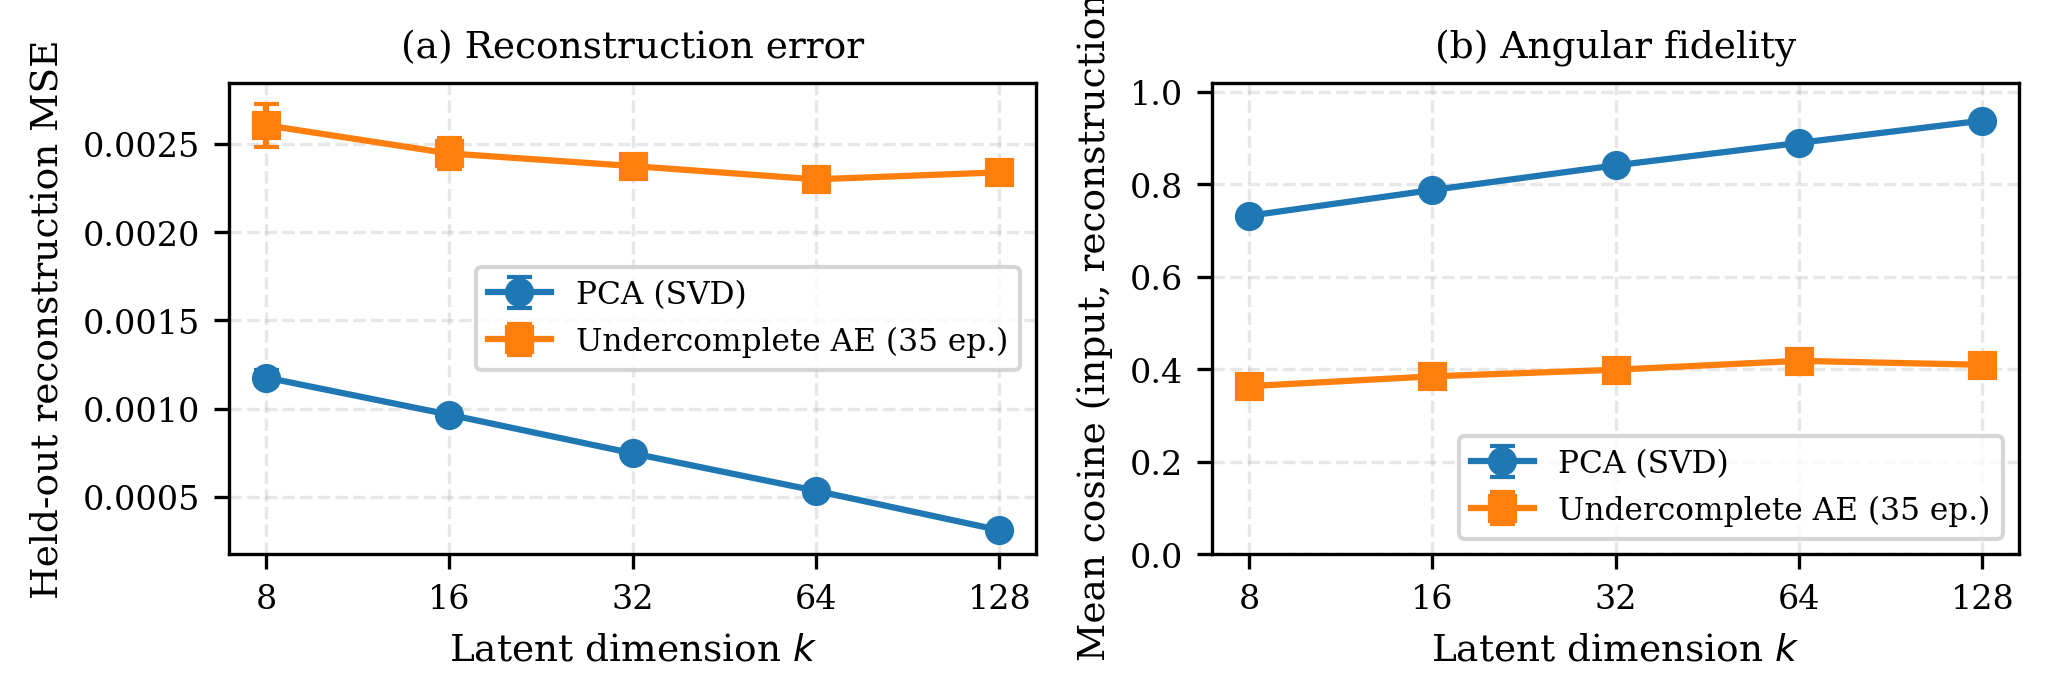
\includegraphics[width=0.92\textwidth]{figures/fig3_pca_vs_ae.png}
\caption{Held-out reconstruction versus latent dimension $k$ for PCA and the deployed undercomplete autoencoder: (a) mean squared error and (b) mean cosine similarity between inputs and reconstructions. Error bars show one standard deviation over five splits.}
\label{fig:pcaae}
\end{figure*}
\begin{figure*}[!t]
\centering
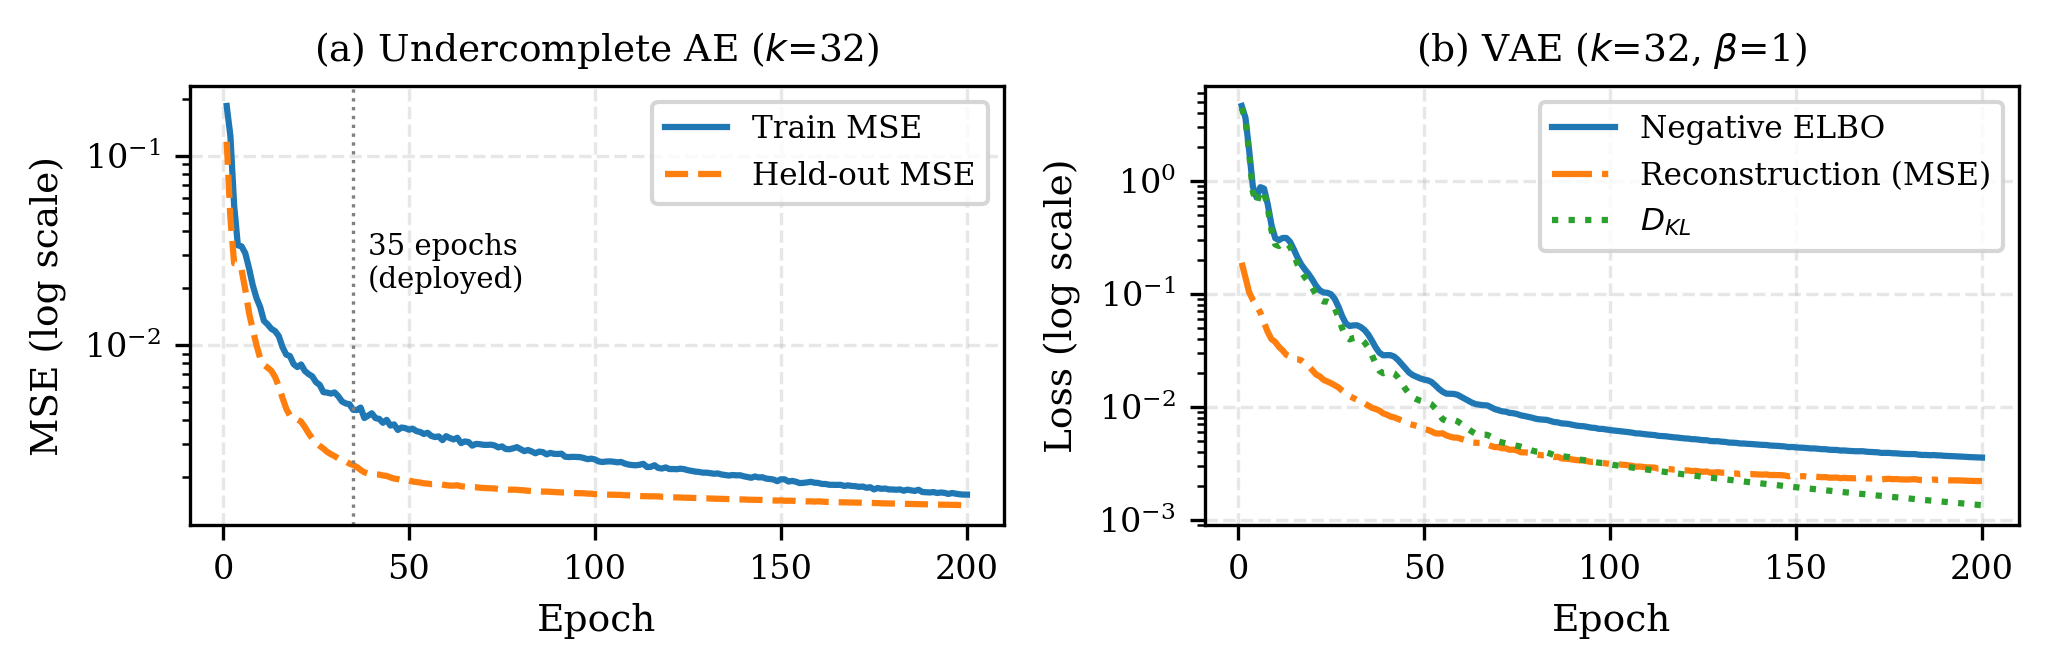
\includegraphics[width=0.92\textwidth]{figures/fig4_training_dynamics.png}
\caption{Training dynamics at $k=32$: (a) undercomplete autoencoder training and held-out MSE, with the deployed 35-epoch budget marked (training loss is higher because dropout is active during training); (b) VAE negative ELBO with its reconstruction and KL components.}
\label{fig:train}
\end{figure*}
Table~\ref{tab:repro} compares these measurements with the figures reported in the project README. The direction of the comparison is the same, but the absolute values differ because the README figures were computed in-sample on 48 vectors with an unrecorded device, whereas Table~\ref{tab:pca} uses held-out data. The README training time of 452\,ms was not reproduced on the CPU, and the README's explained-variance target of at least 85\% at $k=32$ is not met on this corpus.

\begin{table}[!t]
\centering
\caption{Project-reported values (README) versus values reproduced in this study at $k=32$.}
\label{tab:repro}
\footnotesize
\setlength{\tabcolsep}{4pt}
\begin{tabular}{lcc}
\toprule
Quantity & README & This study \\
\midrule
PCA reconstruction MSE & 0.000502 & 0.000747 \\
AE reconstruction MSE & 0.002902 & 0.002374 \\
PCA cosine fidelity & 0.8983 & 0.8408 \\
AE cosine fidelity & 0.1600 & 0.3988 \\
PCA time (ms) & 4.73 & 4.59 \\
AE training time (ms) & 452.03 & 33.42 \\
Samples / evaluation & 48 / in-sample & 202 train, 51 held-out \\
\bottomrule
\end{tabular}
\end{table}
\subsection{RQ2: Out-of-Distribution Detection}
Table~\ref{tab:ood} reports AUROC values. All three detectors separated off-topic from in-domain probe queries almost perfectly. Detecting chunks from a different course was harder: the PCA residual achieved an AUROC of 0.988, clearly above the autoencoder (0.912) and the centroid distance (0.904). Fig.~\ref{fig:ood} shows the autoencoder error distributions. The deployed $3\sigma$ rule is conservative: it flagged about 3\% of in-domain chunks and queries, but only 22.9\% of the cross-course chunks and 84.8\% of the off-topic queries. Because the service additionally requires a top retrieval similarity below 0.28 before intercepting a query, the end-to-end interception rate can only be lower than the rates in Table~\ref{tab:ood}; it was not measured separately. The autoencoder forward pass for one query took a median of 0.035\,ms, excluding query embedding, which retrieval requires in any case.

\begin{table}[!t]
\centering
\caption{OOD detection (mean $\pm$ s.d. over five seeds). Top: AUROC for cross-course chunks (51 held-out ID vs. 62 OOD) and probe queries (25 ID vs. 25 OOD). Bottom: rates of the deployed $3\sigma$ rule.}
\label{tab:ood}
\footnotesize
\setlength{\tabcolsep}{4pt}
\begin{tabular}{lcc}
\toprule
Detector / data & Chunks & Queries \\
\midrule
AE reconstruction error & 0.912 $\pm$ 0.012 & 0.990 $\pm$ 0.006 \\
PCA residual ($k$=32) & 0.988 $\pm$ 0.008 & 0.999 $\pm$ 0.001 \\
Centroid cosine distance & 0.904 $\pm$ 0.024 & 0.998 $\pm$ 0.001 \\
\midrule
Held-out BDA chunks (ID) & FPR & 3.1\% $\pm$ 1.0\% \\
APDD chunks (OOD) & TPR & 22.9\% $\pm$ 10.3\% \\
In-domain queries & FPR & 3.2\% $\pm$ 4.7\% \\
Off-topic queries & TPR & 84.8\% $\pm$ 3.9\% \\
\bottomrule
\end{tabular}
\end{table}
\begin{figure*}[!t]
\centering
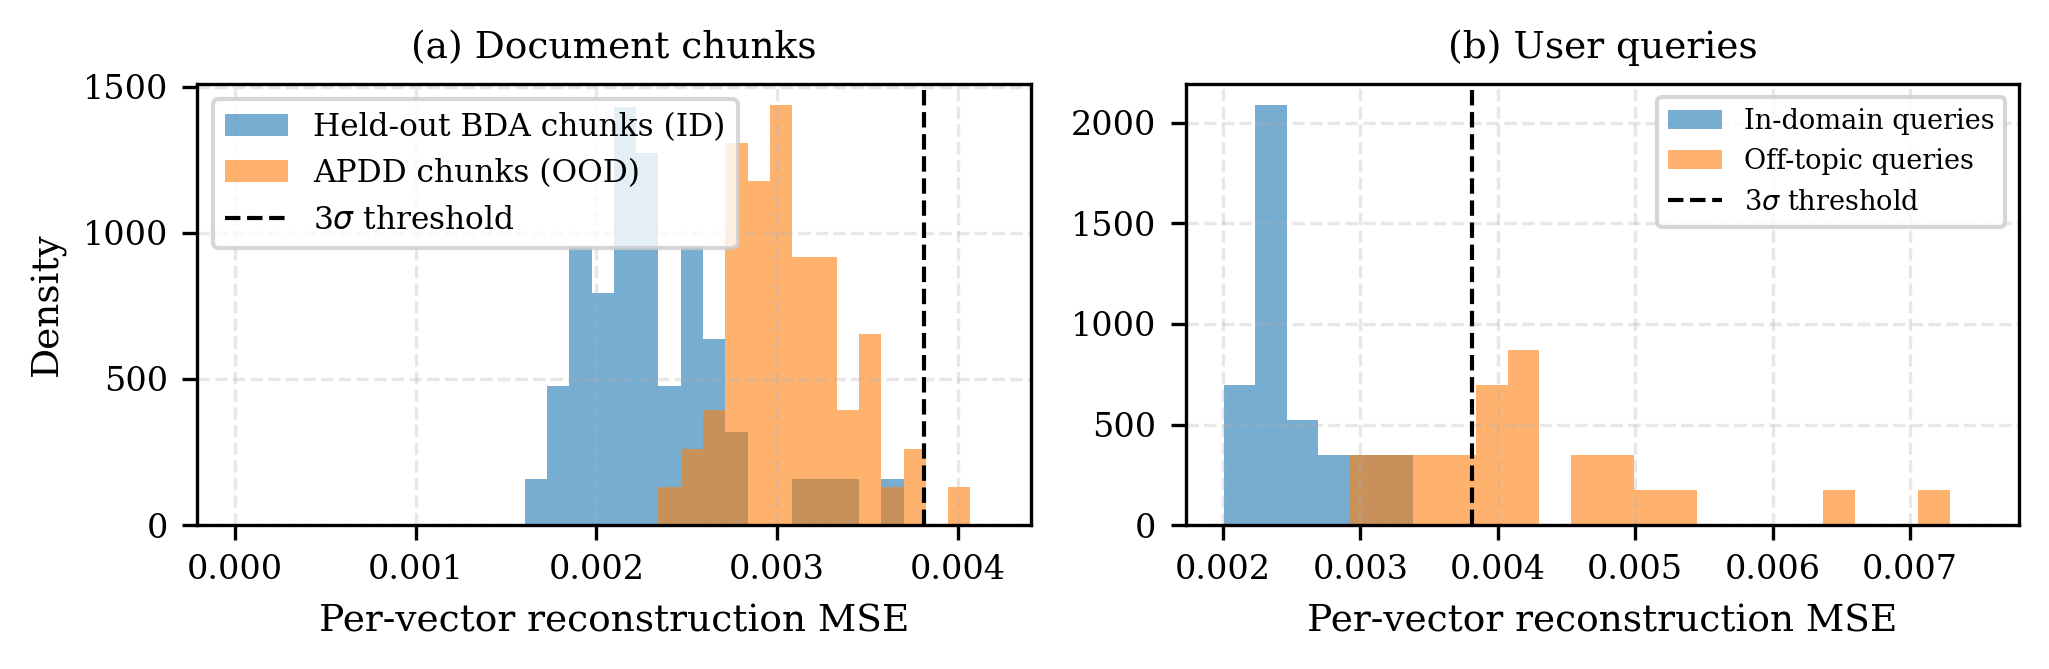
\includegraphics[width=0.92\textwidth]{figures/fig5_ood_detection.png}
\caption{Autoencoder reconstruction error (seed 0) for (a) held-out in-domain chunks versus chunks from another course and (b) in-domain versus off-topic probe queries. The dashed line is the deployed $3\sigma$ threshold.}
\label{fig:ood}
\end{figure*}
\subsection{RQ3: Grounded Answer Refinement}
Table~\ref{tab:ref} reproduces the summary of the five-question benchmark and adds averages over the four answerable questions. Over all five questions, the pipeline had the highest token F1 and ROUGE-L and an UER of zero, while the vanilla FLAN-T5 baseline had a mean UER of 0.20. The per-case breakdown in Fig.~\ref{fig:case} shows that the aggregate advantage comes from the unanswerable question, where the pipeline's abstention message matched the reference exactly (F1 = 1.0) and both baselines scored zero. On the four answerable questions, the pipeline had the lowest token F1 (0.413 vs. 0.532 for direct extraction and 0.463 for vanilla FLAN-T5) and the lowest ROUGE-L. The baseline's UER of 0.20 corresponds to a single question. Moreover, the pipeline's answer to the applications question begins with ``Aircraft'' where the source reads ``Airlines''; this substitution is not counted by the UER because the entity extractor ignores single capitalized words. Mean latency was 1{,}211\,ms for the pipeline and 1{,}065\,ms for the vanilla baseline.

\begin{table*}[!t]
\centering
\caption{Answer-refinement benchmark (project evaluation report). Columns 2--7 average all five questions; the last two columns average the four answerable questions. Latency in milliseconds.}
\label{tab:ref}
\footnotesize
\setlength{\tabcolsep}{4pt}
\begin{tabular}{lcccccccc}
\toprule
System & F1 & ROUGE-L & Fact. cons. & Struct. & UER & Latency & F1 (4) & ROUGE-L (4) \\
\midrule
Direct extraction & 0.426 & 0.371 & 1.000 & 0.96 & 0.00 & 0 & 0.532 & 0.464 \\
Vanilla FLAN-T5 & 0.370 & 0.314 & 0.767 & 0.87 & 0.20 & 1065 & 0.463 & 0.392 \\
Proposed pipeline & 0.530 & 0.481 & 0.780 & 0.88 & 0.00 & 1211 & 0.413 & 0.352 \\
\bottomrule
\end{tabular}
\end{table*}
\begin{figure}[!t]
\centering
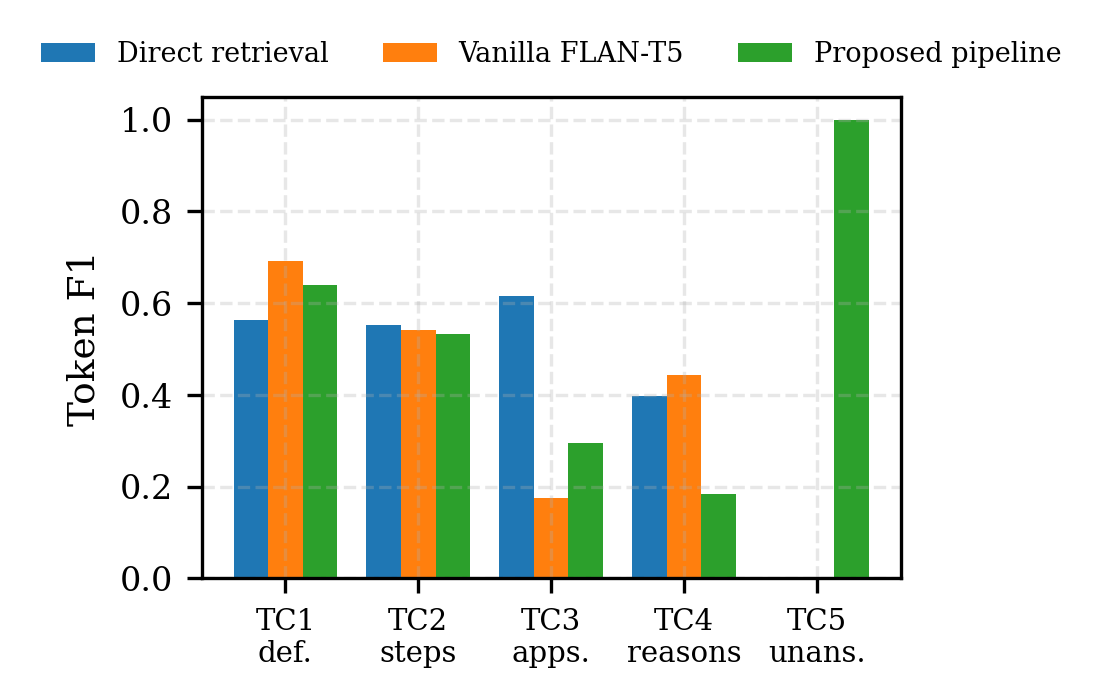
\includegraphics[width=\columnwidth]{figures/fig7_refinement_per_case.png}
\caption{Token F1 per benchmark question. TC5 is unanswerable from the supplied evidence; the reference answer is the system's abstention message.}
\label{fig:case}
\end{figure}
\subsection{RQ4: Distractor Similarity Band}
Fig.~\ref{fig:distr} shows the distribution of pairwise cosine similarities among the 203 section-title concepts (mean 0.157, s.d. 0.150). Of all pairs, 80.9\% fall below the lower bound of 0.25, 19.0\% fall inside the band, and 0.05\% exceed 0.92. For title-level concepts the lower bound is therefore the binding constraint, and the upper bound rarely applies. No human or psychometric evaluation of the generated items was performed, so these results describe the geometry of the candidate space rather than the quality of the questions.

\begin{figure}[!t]
\centering
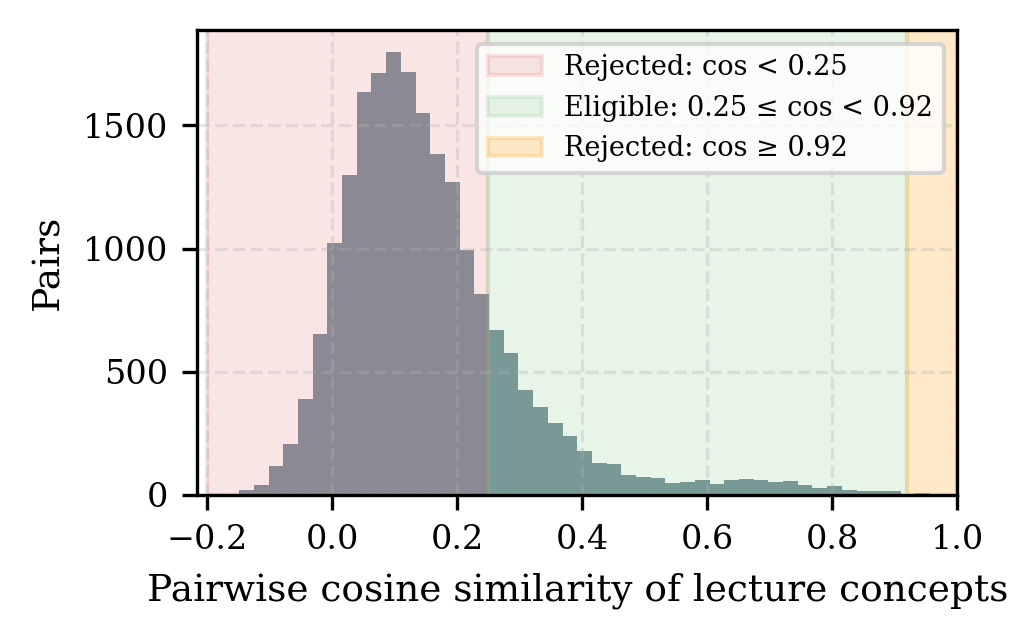
\includegraphics[width=\columnwidth]{figures/fig6_distractor_similarity.png}
\caption{Pairwise cosine similarity among 203 lecture concepts with the implemented distractor band $[0.25, 0.92)$.}
\label{fig:distr}
\end{figure}
\subsection{Software Verification and Documentation Audit}
The automated test suite contains 104 tests in 13 modules (Table~\ref{tab:tests}); all 104 passed in 45.97\,s in the environment described in Section~V-C. The tests verify functional behavior, such as latent dimensions, KL non-negativity, distractor uniqueness, citation preservation, and user isolation; they do not measure learning outcomes. Table~\ref{tab:audit} lists discrepancies between the project README and the code that were found while preparing this paper; the paper describes the implemented behavior throughout.

\begin{table}[!t]
\centering
\caption{Automated tests by module.}
\label{tab:tests}
\footnotesize
\setlength{\tabcolsep}{4pt}
\begin{tabular}{llc}
\toprule
Area & Module & Tests \\
\midrule
Autoencoders, PCA benchmark, OOD & test\_atml\_autoencoders & 14 \\
Quiz anchors and distractors & test\_atml\_quiz\_generation & 18 \\
Incremental knowledge integration & test\_incremental\_knowledge\_integration & 13 \\
Answer refinement and grounding & test\_atml\_refinement & 11 \\
Semantic search and isolation & test\_semantic\_search & 9 \\
Notes generation & test\_atml\_notes\_generation & 8 \\
Notes subtopics and filtering & test\_atml\_notes\_subtopics & 8 \\
Chat normalization and coreference & test\_chatbot\_upgrade & 8 \\
Multimodal retrieval & test\_multimodal\_rag & 5 \\
Storage and validation & test\_storage\_and\_models & 4 \\
Extraction service & test\_extraction\_service & 3 \\
API integration & test\_api\_integration & 2 \\
End-to-end PDF extraction & test\_real\_extraction\_pipeline & 1 \\
\textbf{Total} & 13 modules & \textbf{104} \\
\bottomrule
\end{tabular}
\end{table}
\begin{table*}[!t]
\centering
\caption{Discrepancies between the project documentation and the implementation.}
\label{tab:audit}
\footnotesize
\setlength{\tabcolsep}{4pt}
\begin{tabular}{lll}
\toprule
Item & README & Implementation \\
\midrule
OOD threshold & $\mu + 2.5\sigma$ & $\bar{e} + 3\max(s_e, 5{\times}10^{-4})$ or $z \geq 3$ \\
LeakyReLU slope & 0.1 & 0.2 \\
FLAN-T5 attention heads & 8 & 6 (FLAN-T5-small: 8+8 layers, $d$=512) \\
Distractor band & [0.35, 0.92) & [0.25, 0.92); docstring states [0.40, 0.85] \\
Grounding rejection & any unsupported entity & ratio $>0.45$ with $\geq 2$ entities, or $\rho<0.35$, or $c<0.40$ \\
Denoising AE in ingestion & applied to OCR text & implemented and unit-tested; not called in ingestion path \\
Explained variance at $k$=32 & $\geq 85\%$ & 75.1\% (training split) \\
Quiz distractors & non-generative & FLAN-T5 used as a fallback when the pool is insufficient \\
\bottomrule
\end{tabular}
\end{table*}
\section{Discussion}
\emph{Linear versus nonlinear compression.} The PCA result is consistent with theory: PCA is the optimal linear reconstructor \cite{eckart1936}, and an autoencoder can surpass it only by exploiting nonlinear structure \cite{baldi1989}. With 202 training vectors and a model of roughly $1.1\times10^5$ parameters trained for 35 full-batch steps, no such advantage was observed. For a per-folder detector that must be retrained whenever documents change, the closed-form PCA residual is cheaper, deterministic, and, in this study, more accurate. The autoencoder remains a reasonable design if it is trained to convergence with a validation criterion, but its benefit must be demonstrated rather than assumed.

\emph{Scope detection.} Reconstruction error is a useful and inexpensive signal for off-topic queries, which is the case that matters most for the user interface. The low TPR of the fixed $3\sigma$ rule on cross-course chunks indicates that the threshold, rather than the score, limits performance; a threshold calibrated on a validation set would allow an explicit trade-off between false alarms and missed detections.

\emph{Grounding and refinement.} The measured benefit of the grounded pipeline is concentrated in abstention, which is valuable for a study tool because it avoids answering from outside the course. The evidence does not show that FLAN-T5-small refinement improves lexical agreement on answerable questions; in this benchmark it reduced it. The grounding check is transparent and cheap, but it can reject legitimate paraphrases through the overlap threshold and can accept substitutions such as the one observed in TC3. A zero UER on five questions should therefore be read as an observation on this test set under this metric, not as a guarantee.

\emph{Distractor selection.} The band encodes a sensible design rationale, plausible but non-equivalent options, and its geometry is easy to inspect. Whether it produces items of appropriate difficulty and discrimination is a hypothesis that requires evaluation with students.

\section{Limitations and Threats to Validity}
\begin{itemize}
\item \emph{Corpus size.} Embedding experiments use one folder of 253 chunks from a single subject and one OOD course; results may not transfer to other subjects or larger collections.
\item \emph{Benchmark size.} The answer-refinement benchmark has five questions, one of which is unanswerable; no statistical significance can be claimed, and single cases dominate the averages.
\item \emph{References and metrics.} Reference answers were written by the project authors, and token F1 and ROUGE-L penalize valid paraphrases. The UER shares its entity extractor with the grounding check and misses single-word and lowercase substitutions.
\item \emph{Strict grounding.} The overlap threshold may reject correct paraphrased answers; this effect was not measured.
\item \emph{Embedding dependence.} Retrieval, OOD detection, and distractor selection all depend on the quality of all-MiniLM-L6-v2 embeddings for technical vocabulary.
\item \emph{Probe queries.} The 50 probe queries were written by the authors and may be easier to separate than real student queries.
\item \emph{Hardware.} Latencies depend on hardware and software versions; E5 latencies were recorded on unreported hardware.
\item \emph{Educational effectiveness.} Passing software tests does not establish learning benefits; no user study was conducted.
\item \emph{Replication.} All experiments were run by the authors on their own system; no independent replication has been performed.
\end{itemize}
\section{Conclusion and Future Work}
This paper presented Nalanda AI, a locally hosted study workspace that combines dense retrieval, grounded FLAN-T5 refinement with extractive fallback and abstention, autoencoder-based scope detection, and cosine-constrained distractor selection behind a four-view user interface. On real lecture embeddings, PCA outperformed the deployed autoencoder in held-out reconstruction and cross-course detection, while both separated off-topic queries reliably. On a small answer-refinement benchmark, the grounded pipeline abstained correctly and produced no unsupported entities under the project metric, but it did not improve lexical agreement on answerable questions. Future work should (i) build a larger benchmark spanning several subjects with independently written references; (ii) add human evaluation of answer faithfulness and of quiz item quality, including difficulty and discrimination; (iii) run ablations that isolate the structurer, the generator, and the grounding check; (iv) calibrate OOD thresholds on validation data and compare PCA-residual and converged autoencoder detectors; (v) test robustness to OCR noise; and (vi) report latency on a documented set of edge devices.

\begin{thebibliography}{30}
\bibitem{roediger2006} H. L. Roediger and J. D. Karpicke, ``Test-enhanced learning: Taking memory tests improves long-term retention,'' \emph{Psychol. Sci.}, vol. 17, no. 3, pp. 249--255, 2006.
\bibitem{rozenblit2002} L. Rozenblit and F. Keil, ``The misunderstood limits of folk science: An illusion of explanatory depth,'' \emph{Cogn. Sci.}, vol. 26, no. 5, pp. 521--562, 2002.
\bibitem{lewis2020} P. Lewis \emph{et al.}, ``Retrieval-augmented generation for knowledge-intensive NLP tasks,'' in \emph{Proc. Adv. Neural Inf. Process. Syst. (NeurIPS)}, vol. 33, 2020, pp. 9459--9474.
\bibitem{gao2023} Y. Gao \emph{et al.}, ``Retrieval-augmented generation for large language models: A survey,'' \emph{arXiv preprint arXiv:2312.10997}, 2023.
\bibitem{maynez2020} J. Maynez, S. Narayan, B. Bohnet, and R. McDonald, ``On faithfulness and factuality in abstractive summarization,'' in \emph{Proc. 58th Annu. Meeting Assoc. Comput. Linguistics (ACL)}, 2020, pp. 1906--1919.
\bibitem{ji2023} Z. Ji \emph{et al.}, ``Survey of hallucination in natural language generation,'' \emph{ACM Comput. Surv.}, vol. 55, no. 12, Art. no. 248, 2023.
\bibitem{mitkov2003} R. Mitkov and L. A. Ha, ``Computer-aided generation of multiple-choice tests,'' in \emph{Proc. HLT-NAACL Workshop Building Educational Applications Using Natural Language Processing}, 2003, pp. 17--22.
\bibitem{kurdi2020} G. Kurdi, J. Leo, B. Parsia, U. Sattler, and S. Al-Emari, ``A systematic review of automatic question generation for educational purposes,'' \emph{Int. J. Artif. Intell. Educ.}, vol. 30, no. 1, pp. 121--204, 2020.
\bibitem{karpukhin2020} V. Karpukhin \emph{et al.}, ``Dense passage retrieval for open-domain question answering,'' in \emph{Proc. Conf. Empirical Methods Natural Lang. Process. (EMNLP)}, 2020, pp. 6769--6781.
\bibitem{reimers2019} N. Reimers and I. Gurevych, ``Sentence-BERT: Sentence embeddings using Siamese BERT-networks,'' in \emph{Proc. EMNLP-IJCNLP}, 2019, pp. 3982--3992.
\bibitem{wang2020} W. Wang, F. Wei, L. Dong, H. Bao, N. Yang, and M. Zhou, ``MiniLM: Deep self-attention distillation for task-agnostic compression of pre-trained transformers,'' in \emph{Proc. Adv. Neural Inf. Process. Syst. (NeurIPS)}, vol. 33, 2020, pp. 5776--5788.
\bibitem{vaswani2017} A. Vaswani \emph{et al.}, ``Attention is all you need,'' in \emph{Proc. Adv. Neural Inf. Process. Syst. (NeurIPS)}, vol. 30, 2017, pp. 5998--6008.
\bibitem{raffel2020} C. Raffel \emph{et al.}, ``Exploring the limits of transfer learning with a unified text-to-text transformer,'' \emph{J. Mach. Learn. Res.}, vol. 21, no. 140, pp. 1--67, 2020.
\bibitem{shaw2018} P. Shaw, J. Uszkoreit, and A. Vaswani, ``Self-attention with relative position representations,'' in \emph{Proc. NAACL-HLT}, 2018, pp. 464--468.
\bibitem{chung2024} H. W. Chung \emph{et al.}, ``Scaling instruction-finetuned language models,'' \emph{J. Mach. Learn. Res.}, vol. 25, no. 70, pp. 1--53, 2024.
\bibitem{pearson1901} K. Pearson, ``On lines and planes of closest fit to systems of points in space,'' \emph{Philos. Mag.}, vol. 2, no. 11, pp. 559--572, 1901.
\bibitem{jolliffe2016} I. T. Jolliffe and J. Cadima, ``Principal component analysis: A review and recent developments,'' \emph{Philos. Trans. Roy. Soc. A}, vol. 374, no. 2065, Art. no. 20150202, 2016.
\bibitem{eckart1936} C. Eckart and G. Young, ``The approximation of one matrix by another of lower rank,'' \emph{Psychometrika}, vol. 1, no. 3, pp. 211--218, 1936.
\bibitem{baldi1989} P. Baldi and K. Hornik, ``Neural networks and principal component analysis: Learning from examples without local minima,'' \emph{Neural Netw.}, vol. 2, no. 1, pp. 53--58, 1989.
\bibitem{hinton2006} G. E. Hinton and R. R. Salakhutdinov, ``Reducing the dimensionality of data with neural networks,'' \emph{Science}, vol. 313, no. 5786, pp. 504--507, 2006.
\bibitem{kingma2014} D. P. Kingma and M. Welling, ``Auto-encoding variational Bayes,'' in \emph{Proc. Int. Conf. Learn. Represent. (ICLR)}, 2014.
\bibitem{vincent2008} P. Vincent, H. Larochelle, Y. Bengio, and P.-A. Manzagol, ``Extracting and composing robust features with denoising autoencoders,'' in \emph{Proc. 25th Int. Conf. Mach. Learn. (ICML)}, 2008, pp. 1096--1103.
\bibitem{chandola2009} V. Chandola, A. Banerjee, and V. Kumar, ``Anomaly detection: A survey,'' \emph{ACM Comput. Surv.}, vol. 41, no. 3, Art. no. 15, 2009.
\bibitem{sakurada2014} M. Sakurada and T. Yairi, ``Anomaly detection using autoencoders with nonlinear dimensionality reduction,'' in \emph{Proc. 2nd Workshop Mach. Learn. Sensory Data Anal. (MLSDA)}, 2014, pp. 4--11.
\bibitem{hendrycks2017} D. Hendrycks and K. Gimpel, ``A baseline for detecting misclassified and out-of-distribution examples in neural networks,'' in \emph{Proc. Int. Conf. Learn. Represent. (ICLR)}, 2017.
\bibitem{rajpurkar2016} P. Rajpurkar, J. Zhang, K. Lopyrev, and P. Liang, ``SQuAD: 100,000+ questions for machine comprehension of text,'' in \emph{Proc. Conf. Empirical Methods Natural Lang. Process. (EMNLP)}, 2016, pp. 2383--2392.
\bibitem{lin2004} C.-Y. Lin, ``ROUGE: A package for automatic evaluation of summaries,'' in \emph{Text Summarization Branches Out}, 2004, pp. 74--81.
\bibitem{ba2016} J. L. Ba, J. R. Kiros, and G. E. Hinton, ``Layer normalization,'' \emph{arXiv preprint arXiv:1607.06450}, 2016.
\bibitem{kingma2015} D. P. Kingma and J. Ba, ``Adam: A method for stochastic optimization,'' in \emph{Proc. Int. Conf. Learn. Represent. (ICLR)}, 2015.
\bibitem{fawcett2006} T. Fawcett, ``An introduction to ROC analysis,'' \emph{Pattern Recognit. Lett.}, vol. 27, no. 8, pp. 861--874, 2006.
\end{thebibliography}
\end{document}